\documentclass[11pt]{article}
\usepackage[utf8]{inputenc}
\usepackage[english]{babel}
\usepackage{amssymb}
\usepackage{environ}
\usepackage{amsthm} 
\usepackage{amsmath}
\usepackage{bbm}
\usepackage{mathtools}
\usepackage{fullpage}
\usepackage{comment}
\usepackage{graphicx}
\usepackage{tikz}
\newcommand{\Or}{\mbox{ OR }}
\newcommand{\AND}{\mbox{ AND }}
\newcommand{\Not}{\mbox{NOT}}
\newcommand{\Iff}{\mbox{ IFF }}
\newcommand{\True}{\mbox{T}}
\newcommand{\False}{\mbox{F}}
\setlength{\parskip}{0ex}
\newcommand{\Implies}{\mbox{ IMPLIES }}
\newcommand{\proot}[2]{\sqrt[\leftroot{-3}\uproot{3}#1]{#2}}
\newcommand{\ints}{\mathbb{Z}}
\newcommand{\nats}{\mathbb{N}}
\newcommand{\rats}{\mathbb{Q}}
\newcommand{\comps}{\mathbb{C}}
\newcommand{\reals}{\mathbb{R}}
\newcommand{\field}{\mathbb{F}}
\newcommand{\pints}{\mathcal{P}(\mathbb{Z})}
\newcommand{\pnats}{\mathcal{P}(\mathbb{N})}
\newcommand{\prats}{\mathcal{P}(\mathbb{Q})}
\newcommand{\pcomps}{\mathcal{P}(\mathbb{C})}
\newcommand{\preals}{\mathcal{P}(\mathbb{R})}
\newcommand{\pfield}{\mathcal{P}(\mathbb{F})}
\newcommand{\half}{\frac{1}{2}}
\newcommand{\abs}[1]{\left\lvert #1 \right\rvert}%
\newcommand{\norm}[1]{\left\lVert #1 \right\rVert}%
\newcommand{\interior}{\text{int}}
\newcommand{\halfe}{\frac{\epsilon}{2}}
\newcommand{\id}{\text{Id}}

\title{Control Systems}
\author{Rein}
\date{\today}


\begin{document}
	\maketitle
	\tableofcontents

\section{Laplace Transform}
\subsection{Definition: $\mathcal{L}(f(t)) = F(s) = \int_{0-}^{\infty} e^{-st}f(t) dt$ where $s = \sigma + j \omega \in \comps$. }
\subsection{Inverse: $\mathcal{L}^{-1}(F(s)) = f(t)u(t) =  \frac{1}{2 \pi j}\int_{\sigma - j \infty}^{\sigma + j \infty} e^{st} F(s) ds $ where $s = \sigma + j \omega \in \comps$ and $u(t) = \begin{cases}
		1 & t > 0 \\ 0 & t < 0
\end{cases}$}

\subsection{Common Transforms}
\subsubsection{$f(t) = \delta(t) \implies F(s) = 1$}
\begin{proof}
	

	Dirac-$\delta$ function: $\delta(t) =  0$ if $ t > 0 $ and defined as
	$\int_{\reals} h(t) \delta(t) dt = h(0)$. Equivalently, defined as the non-functional limit 
	\[\lim_{T \to \infty} T_p(t)\] where \[T_p = \begin{cases}
		0 & \abs{t} \geq \frac{1}{T} \\ \frac{1}{2}T & \abs{t} < \frac{1}{T}
	\end{cases}\] This is not a function since $\lim_{T \to \infty} T_p(0) \to \infty$. Also,
\[\int_{\reals} h(t) \lim_{T \to \infty} T_p(t) dt = \lim_{T \to \infty} \int_{\reals} h(t)  T_p(t)  dt \]\[=  \lim_{T \to \infty} \lim_{n \to \infty} \sum_{k = 1}^{n} h(\frac{-1}{T} + k \frac{2}{Tn})\frac{1}{2}T \frac{2}{Tn} =  \lim_{T \to \infty} \lim_{n \to \infty}\sum_{k = 1}^{n} h(\frac{-1}{T} + k \frac{2}{Tn}) \frac{1}{n} \]\[=  \lim_{n \to \infty} \sum_{k = 1}^n h(0) \frac{1}{n} = \lim_{n \to \infty}h(0) = h(0) \] by definition of the Riemann integral. Realize also that 
\[\lim_{T \to \infty} \int_{0}^{\infty} h(t)  T_p(t)  dt = \lim_{T \to \infty} \lim_{n \to \infty} \sum_{k = 1}^{n} h( k \frac{2}{Tn})\frac{1}{2}T \frac{2}{Tn} = h(0)\]
and the same holds true for the integral on the left half-plane. 

Thus the Laplace transform is
\[\mathcal{L}(\delta(t))(s) = F(s) = \int_{0-}^{\infty} e^{-st}\delta(t)  dt = e^{-s0} = 1 \]
\end{proof}

\subsubsection{$f(t) = u(t) \implies F(s) = \frac{1}{s}$}
\begin{proof}
Unit step function: $u(t) = \begin{cases}
	0 & t < 0 \\ 1 & t > 0
\end{cases}$

\[\mathcal{L}(u(t))(s) = F(s) = \int_{0-}^{\infty} e^{-st}u(t)  dt  = \int_{0-}^{\infty} e^{-st} dt = 0-\frac{-1}{s}e^0 = \frac{1}{s}\]
\end{proof}


\subsubsection{$f(t) = tu(t) \implies F(s) = \frac{1}{s^2}$}
\begin{proof}


\[\mathcal{L}(tu(t))(s) = F(s) = \int_{0-}^{\infty} e^{-st}tu(t)  dt  = \int_{0-}^{\infty} te^{-st} dt = t\frac{-1}{s}e^{-st} - \int \frac{-1}{s} e^{-st}\]
\[= \lim_{t \to \infty} \frac{-1}{s} \frac{t}{e^{st}} + \frac{1}{s^2} = \frac{1}{s^2}\]

	
\end{proof}

\subsubsection{$f(t) = t^n u(t) \implies F(s)  = \frac{(n + 1)!}{s^{n + 2}} $}
\begin{proof}

Assume by induction $\mathcal{L}(t^nu(t))(s) = \frac{n!}{s^{n + 1}}$ which holds for $n =  0, 1$. Then 
\[\mathcal{L}(t^{n + 1}u(t))(s) = F(s) =  \int_{0-}^{\infty} t^{n + 1}e^{-st} dt  = t^{n + 1} \frac{-1}{s}e^{- st} - \int (n + 1) t^n \frac{-1}{s} e^{-st}\]
\[= \frac{1}{s} (n + 1) \frac{n!}{s^{n + 1}} = \frac{(n + 1)!}{s^{n + 2}} \]
	
\end{proof}
\subsubsection{$f(t) = e^{-at}u(t) \implies F(s)  = \frac{1}{s + a}$}
\begin{proof}

\[\mathcal{L}(e^{-at}u(t))(s) = F(s) = \int_{0-}^{\infty} e^{-st}e^{-at}u(t)  dt =  \int_{0-}^{\infty} e^{-(s + a)t} dt = \frac{1}{s + a}\]
	
\end{proof}
\subsubsection{$f(t) =  \sin \omega t u(t) \implies F(s)  = \frac{\omega}{s^2 + \omega^2}$}
\begin{proof}

\[\mathcal{L}(\sin \omega t u(t))(s) = F(s) = \int_{0-}^{\infty} e^{-st}\sin \omega tu(t)  dt \]
\[\int_0^{\infty} e^{-st} \frac{e^{i\omega t} - e^{-i\omega t}}{2i} dt = \frac{1}{2i} \int_0^{\infty}  e^{(-s + i \omega)t} - e^{(-s - i\omega)t} dt = \]
\[= \frac{1}{2i} (\frac{1}{s - i \omega} - \frac{1}{s + i \omega}) = \frac{1}{2i} \frac{2i \omega}{s^2 + \omega^2}= \frac{\omega}{s^2 + \omega^2}\]
	
\end{proof}


\subsubsection{$f(t) = \cos \omega t u(t) \implies F(s)  = \frac{s}{s^2 + \omega^2}$}
\begin{proof}

\[\mathcal{L}(\cos \omega t u(t))(s) = F(s) = \int_{0-}^{\infty} e^{-st}\cos \omega tu(t)  dt \]
\[\int_0^{\infty} e^{-st} \frac{e^{i\omega t} + e^{-i\omega t}}{2} dt = \frac{1}{2} \int_0^{\infty}  e^{(-s + i \omega)t} + e^{(-s - i\omega)t} dt = \]
\[= \frac{1}{2} (\frac{1}{s - i \omega} + \frac{1}{s + i \omega}) = \frac{1}{2} \frac{2s}{s^2 + \omega^2}= \frac{s}{s^2 + \omega^2}\]
	
\end{proof}

\subsection{Common Theorems}
\subsubsection{Frequency Shift Theorem: $\mathcal{L}(e^{-at}f(t)) = F(s + a)$}
\begin{proof}
	\[\mathcal{L}(e^{-at}f(t)) = \int_0^{\infty} e^{-st}e^{-at}f(t) dt = \int_0^{\infty} e^{-(s + a)t}f(t) dt = F(s + a)\]
\end{proof}

\subsubsection{Time Shift Theorem: $\mathcal{L}(f(t - T)) = e^{-sT}F(s)$}
\begin{proof}
	\[\mathcal{L}(f(t - T)) = \int_0^{\infty} e^{-st} f(t - T) dt
\] 
	\[ = e^{-sT}\int_{0}^{\infty}e^{-st + sT} f(t - T) dt =e^{-sT}\int_{0}^{\infty}e^{-s(t - T)} f(t - T) dt\]
	\[=e^{-sT}\int_{-T}^{\infty}e^{-st} f(t) dt = e^{-sT}f(t)\] where we note $f(t) = f(t)u(t)$ must hold for the final result. 
\end{proof}

\subsubsection{Scaling Theorem: $\mathcal{L}(f(at))  = \frac{1}{a}F(\frac{s}{a})$}

\begin{proof}
	\[\mathcal{L}(f(at))  =  \int_0^{\infty} e^{-st}f(at) dt = \frac{1}{a}\int_0^{\infty} e^{-st'/a}f(t') dt'\]
	\[= \frac{1}{a} F(\frac{s}{a})\] letting $t' = at \implies dt = \frac{1}{a} dt'$.
\end{proof}

\subsubsection{Differentiation Theorem: $\mathcal{L}(\frac{df}{dt}) = sF(s) - f(0-)$}
\begin{proof}
	\[\mathcal{L}(\frac{df}{dt})  = \int_0^{\infty} e^{-st} \frac{df}{dt} dt\]
	\[= e^{-st} f(t) - \int_0^{\infty} -s e^{-st} f(t) dt = - \lim_{t \to 0} f(t) + sF(s)\]
\end{proof}

\subsubsection{Differentiation Theorem: $\mathcal{L}(\frac{d^2f}{dt^2}) = s^2F(s) - sf(0-) - f'(0-)$}

\begin{proof}
	\[\mathcal{L}(\frac{d^2f}{dt^2}) = \int_0^{\infty} e^{-st} \frac{d^2f}{dt^2} dt\]
	\[= e^{-st} f'(t) - \int_0^{\infty} -se^{-st} \frac{df}{dt} dt = -\lim_{t \to 0}f'(t) + s^2F(s) - s\lim_{t \to 0}f(t)\]
\end{proof}

\subsubsection{Differentiation Theorem: $\mathcal{L}(\frac{d^nf}{dt^n}) = s^nF(s) - \sum_{k = 1}^n s^{n - k} f^{k - 1}(0-)$}
\begin{proof}
	Suppose by induction this is true, which is clear for $n = 1, 2$, then 
	\[\mathcal{L}(\frac{d^{n + 1}f}{dt^{n + 1}}) = \int_0^{\infty} e^{-st} \frac{d^{n + 1}f}{dt^{n + 1}} dt\]
	\[ = e^{-st} \frac{d^nf}{dt^n} + s \int_0^{\infty} e^{-st} \frac{d^nf}{dt^n} dt = -\lim_{t\to 0} f^n(t) + s\left( s^nF(s) - \sum_{k = 1}^n s^{n - k} f^{k - 1}(0-)\right) \]
	\[= -\lim_{t\to 0} f^n(t) +  s^{n + 1}F(s) - \sum_{k = 1}^n s^{n + 1 - k} f^{k - 1}(0-) \]
	\[= -s^{(n + 1) - (n + 1)} f^{(n + 1) - 1} (0-)  +  s^{n + 1}F(s) - \sum_{k = 1}^n s^{n + 1 - k} f^{k - 1}(0-) \]
	\[= s^{n + 1}F(s) - \sum_{k = 1}^{n + 1} s^{n + 1 - k} f^{k - 1}(0-)\]
\end{proof}

\subsubsection{Integration Theorem: $\mathcal{L}(\int_{0-}^t f(\tau) d\tau ) = \frac{F(s)}{s}$}
\begin{proof}
	\[\mathcal{L}(\int_{0-}^t f(\tau) d\tau ) =  \int_0^{\infty} e^{-st} \int_{0-}^t f(\tau) d\tau dt\]
	\[= \int_{0-}^t f(\tau) d\tau \frac{-1}{s} e^{-st} - \int_0^{\infty}\frac{-1}{s} e^{-st} f(t) dt = \frac{F(s)}{s}\]
\end{proof}

\subsection{Partial Fraction Decomposition, Real Roots: If $F(s) = \frac{N(s)}{D(s)}$ where $\deg N < \deg D$, then factoring $D = \Pi_{k = 1}^n (s + p_k)^{n_k}$ we have $F(s) = \sum_{k = 1}^n \sum_{l = 1}^{n_k} \frac{A_{k, l}}{(s + p_k)^l}$ by partial fraction decomposition. Letting $F_k = (s + p_k)^{n_k}F$ it follows $A_{m, q} = \lim_{s \to -p_m}\frac{1}{(q - 1)!} \frac{d^{q - 1}F_m(s)}{ds^{q - 1}} $}

\begin{proof}
	\[F_{m}(s) = (s + p_m)^{n_m}F(s) = (s + p_m)^{n_m} \sum_{k = 1}^n \sum_{l = 1}^{n_k} \frac{A_{k, l}}{(s + p_k)^l}\]
	\[=  (s + p_m)^{n_m}\sum_{k \neq m }^n \sum_{l = 1}^{n_k} \frac{A_{k, l}}{(s + p_k)^l} +  \sum_{l = 1}^{n_m} \frac{A_{m, l}}{(s + p_m)^{l - n_m}} \]
	\[=  (s + p_m)^{n_m}\sum_{k \neq m }^n \sum_{l = 1}^{n_k} \frac{A_{k, l}}{(s + p_k)^l} +  \sum_{l = 1}^{n_m} A_{m, l} (s + p_m)^{n_m - l}\]
	Now observe
	\[\frac{d^{q - 1}F_m(s)}{ds^{q - 1}} \]\[= \frac{d^{q - 2}}{ds^{q - 2}}\left[n_m(s + p_m)^{n_m  - 1}\sum_{k \neq m }^n \sum_{l = 1}^{n_k} \frac{A_{k, l}}{(s + p_k)^l} +  (s + p_m)^{n_m} \frac{d}{ds}\left(\sum_{k \neq m }^n \sum_{l = 1}^{n_k} \frac{A_{k, l}}{(s + p_k)^l}\right)\right]\]
	

	\[+  \sum_{l = 1}^{n_m} \Pi_{t = -q + 2}^{0}(n_m - l + t) A_{m, l} (s + p_m)^{n_m - l - q + 1}\]
	
	\[= \frac{d^{q - 2}}{ds^{q - 2}}\left\lbrace (s + p_m)^{n_m  - 1} \left[ n_m \sum_{k \neq m }^n \sum_{l = 1}^{n_k} \frac{A_{k, l}}{(s + p_k)^l}  +  (s + p_m) \frac{d}{ds}\left(\sum_{k \neq m }^n \sum_{l = 1}^{n_k} \frac{A_{k, l}}{(s + p_k)^l}\right)\right] \right\rbrace\]
	
	
	\[+  \sum_{l = 1}^{n_m} \Pi_{t = -q + 2}^{0}(n_m - l + t) A_{m, l} (s + p_m)^{n_m - l - q + 1}\]
	and as $s \to -p_m$ we see the first term vanishes by the chain rule while the third has the only non-zero term occuring at $l = n_m - q + 1$ giving
	\[ \Pi_{t = -q + 2}^{0}(n_m - (n_m - q + 1) + t) A_{m, (n_m - q + 1)} (s + p_m)^{n_m - (n_m - q + 1) - q + 1}\] 
	\[ = \Pi_{t = -q + 2}^{0}(q - 1+ t) A_{m, n_m - q + 1} = (q - 1)!A_{m, n_m - q + 1}  \] 
	Note that here we switched the order of $A_{k, l}$ so that $p_k$ is a root of multiplicity $l$ with residue $A_{k, l}$ (which seems natural); if we write $A_{k, l}$ as the residue of the term with $p_k$ as root of multiplicity $n_k - l + 1$ then we get $ (q - 1)!A_{m, q}$. 
	
\end{proof}

\subsubsection{Complex Roots: If $p_m = \overline{p_o} \in \comps$ then $A_{m, q} = \overline{A_{o, q}}$}
\begin{proof}
	For simplicity in notation switch the ordering of $A_{k, l}$ as mentioned at the end of the previous proof. The use of the above claim is to simplify solving for $A_{o}$ if one knows $A_{m}$. 
	\[A_{o, q} = \lim_{s \to - p_{o, q}} \frac{1}{(q - 1)!}\frac{d^{q - 1}(s + p_o)F(s)}{ds^{q - 1}}= \lim_{s \to -\overline{p_m}} \frac{1}{(q - 1)!}\frac{d^{q - 1}(s + \overline{p_m})F(s)}{ds^{q - 1}}\]
	\[= \lim_{s \to -\overline{p_m}} \frac{1}{(q - 1)!}\frac{d^{q - 1}(s + \overline{p_m})^qF(s)}{ds^{q - 1}}\]
	\[= \lim_{s \to -p_m} \frac{1}{(q - 1)!}\frac{d^{q - 1}(\overline{s} + \overline{p_m})^qF(\overline{s})}{ds^{q - 1}}\]
	Since $F$ is a fraction of polynomials, we have $F(\overline{s}) = \overline{F(s)}$ so 
	\[= \lim_{s \to -p_m} \frac{1}{(q - 1)!}\frac{d^{q - 1}(\overline{s + p_m})^q\overline{F(s)}}{ds^{q - 1}}\]
	\[= \lim_{s \to -p_m} \overline{\frac{1}{(q - 1)!}}\frac{d^{q - 1}\overline{(s + p_m)^q}\overline{F(s)}}{ds^{q - 1}}\]
	\[= \overline{ \lim_{s \to -p_m} \frac{1}{(q - 1)!}\frac{d^{q - 1}(s + p_m)^q}{F(s)}{ds^{q - 1}}} = \overline{A_{m, q}}\]
\end{proof} 

\subsection{Example: $f(t) = te^{-5t} \implies F(s) = \frac{1}{(s + 5)^2}$}
\begin{proof}
	Observe 
	\[\mathcal{L}(te^{-5t}) = \int_0^{\infty} e^{-st} te^{-5t} dt =  \int_0^{\infty} te^{-t(s + 5)} dt\]
	\[= t \frac{-1}{(s + 5)} e^{-t(s + 5)} -  \int_0^{\infty}  \frac{-1}{s + 5} e^{-t(s + 5)} dt\]
	\[= 0 + \frac{1}{s + 5} \mathcal{L}(e^{-5t}u(t)) = \frac{1}{( s + 5)^2}\]
\end{proof}

\subsection{Example: $F(s) = \frac{10}{s(s + 2)(s + 3)^2} \implies f(t) = \frac{5}{9} - 5e^{-2t} + \frac{10}{3}te^{-3t} + \frac{40}{9}e^{-3t}$}
\begin{proof}
	Observe
	\[\frac{10}{s(s + 2)(s + 3)^2} = \frac{A}{s} + \frac{B}{s + 2} + \frac{C}{(s + 3)^2} + \frac{D}{s + 3}\] where
	\[A = \lim_{s \to 0} \frac{10}{(s + 2)(s + 3)^2} = \frac{5}{9}\]
	\[B = \lim_{s \to -2} \frac{10}{s(s + 3)^2} = -5\]
	\[C = \lim_{s \to -3}  \frac{10}{s(s + 2)} = \frac{10}{3} \]
	\[D = \lim_{s \to -3} \frac{d}{ds} \frac{10}{s(s + 2)} = \lim_{s \to -3}  \frac{-10(2s + 2)}{s^2(s + 2)^2}  = \frac{40}{9}\]
	Thus 
	
	\[\mathcal{L}^{-1}(\frac{10}{s(s + 2)(s + 3)^2}) = \mathcal{L}^{-1} \left(\frac{\frac{5}{9}}{s} + \frac{-5}{s + 2} + \frac{\frac{10}{3}}{(s + 3)^2} + \frac{\frac{40}{9}}{s + 3}\right)\]
	\[= \frac{5}{9}\mathcal{L}^{-1} \left( \frac{1}{s}\right) - 5 \mathcal{L}^{-1} \left( \frac{1}{s + 2}\right) + \frac{10}{3} \mathcal{L}^{-1} \left( \frac{1}{(s + 3)^2} \right) + \frac{40}{9}\mathcal{L}^{-1} \left( \frac{1}{s + 3}\right) \]
	\[= \frac{5}{9} - 5e^{-2t} + \frac{10}{3}te^{-3t} + \frac{40}{9}e^{-3t}\]
	
\end{proof}

\clearpage
\section{The Transfer Function}
Let $c(t)$ be the output of a control system, $r(t)$ be the input, and the control system represented by 
\[a_n c^{(n)}(t) + a_{n - 1}c^{(n - 1)}(t) + \ldots a_0c(t) =  b_m r^{(n)}(t) + b_{m - 1}r^{(n - 1)}(t) + \ldots b_0r(t)\] and let $C(s) = \mathcal{L}(c(t)), R(s) = \mathcal{L}(r(t))$ be the transforms. If the initial conditions (including derivatives) of $c$ and $r$ are zero, then applying the Laplace transform to both sides gives
\[a_n s^n C(s) + a_{n - 1}s^{n - 1}C(s) + \ldots a_0C(s) = b_m s^n R(s) + b_{m - 1}s^{m - 1}R(s) + \ldots b_0 R(s)\]
\[\iff G(s) := \frac{C(s)}{R(s)} = \frac{\sum_{k = 0}^m b_k s^k}{\sum_{k = 0}^n a_k s^k}\] where $G$ is the defined transfer function. 

\subsection{Example: The output of the system given by $c'(t) + 2c(t) = r(t)$ with zero initial conditions to the input $r(t) = u(t)$ is $c(t) = \frac{1}{2} - \frac{1}{2}e^{-2t}$.}
\begin{proof}
	The transfer function is
	\[G(s) = \frac{1}{s + 2}\] and $R(s) = \mathcal{L}(u(t)) = \frac{1}{s}$ thus
	\[C(s) = G(s)R(s) = \frac{1}{s(s + 2)}\] 
	Partial fraction decomposition gives
	\[C(s) = \frac{A}{s} + \frac{B}{s + 2}\] where
	\[A = \lim_{s \to 0} \frac{1}{s + 2}  =\frac{1}{2}\]
	\[B = \lim_{s \to -2} \frac{1}{s} = \frac{1}{-2}\] so
	\[c(t) = \mathcal{L}^{-1}(C(s)) = \frac{1}{2}\mathcal{L}^{-1}(\frac{1}{s}) - \frac{1}{2} \mathcal{L}^{-1}(\frac{1}{s + 2}) = \frac{1}{2} - \frac{1}{2}e^{-2t}\]
\end{proof}

\subsection{Example: The ramp response of the system given by $G(s) = \frac{s}{(s + 4)(s + 8)}$ is $c(t) = \frac{1}{32} - \frac{1}{16}e^{-4t} + \frac{1}{32} e^{-8t}$.}

\begin{proof}
	The ramp response is $r(t) = t$ for $t > 0$. Thus
	\[R(s) = \mathcal{L}(r(t)) = \frac{1}{s^2}\] Now
	\[C(s) = G(s)R(s) = \frac{1}{s(s + 4)(s + 8)}\] given by the partial fraction decomposition
	\[C(s) = \frac{A}{s} + \frac{B}{s + 4} + \frac{C}{s + 8}\] where
	\[A = \lim_{s \to 0} \frac{1}{(s + 4)(s + 8)} = \frac{1}{32}\]
	\[B = \lim_{s \to -4} \frac{1}{s(s + 8)} = \frac{1}{-16}\]
	\[C = \lim_{s \to -8} \frac{1}{s(s + 4)} = \frac{1}{32}\] so 
	\[c(t) = \frac{1}{32} \mathcal{L}^{-1}(\frac{1}{s}) - \frac{1}{16} \mathcal{L}^{-1}(\frac{1}{s + 4}) + \frac{1}{32} \mathcal{L}^{-1}(\frac{1}{s + 8}) = \frac{1}{32} - \frac{1}{16}e^{-4t} + \frac{1}{32}e^{-8t}\]
\end{proof}

\section{Electrical Network Transfer Functions}

\subsection{Consider \newline
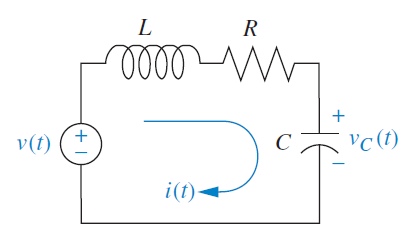
\includegraphics{mesh1.png} containing capacitor with capacitance $C$, resistor with resistance $R$ and inductor with inductance $L$. The transfer function relating the voltage at the capacitor $v_C(t)$ to the applied $v(t)$ is $G(s) = \frac{1}{LCs^2 + CRs + 1}$.}


\subsubsection{Using Kirchhoff's Voltage Law (Mesh Analysis): }
\begin{proof}
	By Kirchhoff's law
	\[v(t) = v_L(t) + v_R(t) + v_C(t) = L i'(t) + Ri(t) + v_C(t)\]
	holds everywhere in the circuit. Now at the capacitor, $v_C(t) = \frac{1}{C} \int_0^t i(\tau) d\tau \implies i(t) = Cv_C'(t)$. Thus, making the substitution gives
	\[ v(t) = LCv''_C(t) + RCv'_C(t) + v_C(t)\]
	In taking the Laplacian (assuming zero initial conditions) we get
	\[G(s) = \frac{1}{LCs^2 + RCs + 1}\]
\end{proof}

\subsubsection{(Transformed): \newline
	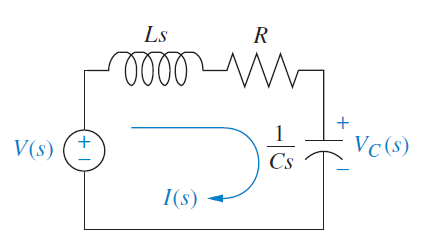
\includegraphics{mesh2.png} }
\begin{proof}
	By Kirchhoff's law
	\[v(t) = v_L(t) + v_R(t) + v_C(t) = L i'(t) + Ri(t) + \frac{1}{C} \int_0^t i(\tau) d\tau \]
	\[\implies V(s) = V_L(s) + V_R(s)+ V_C(s) =  LsI(s) + RI(s) + \frac{1}{Cs}I(s) \]
	where $Z_{\alpha}(s) = \frac{V_{\alpha}(s)}{I(s)}$ are the respective impedances $Ls, R$ and $\frac{1}{Cs}$. Thus 
	\[V(s) = (Ls + R+ \frac{1}{Cs})I(s)\]
	and we obtain
	\[\frac{V_C(s))}{V(s)} = \frac{Z_C(s)I(s)}{(Ls + R+ \frac{1}{Cs})I(s)} =  \frac{1}{Cs (Ls + R+ \frac{1}{Cs})} = \frac{1}{LCs^2 + RCs + 1}\] as the transfer function. 
\end{proof}

\subsubsection{Using Kirchhoff's Current Law (Nodal Analysis)}
\begin{proof}
	By Kirchhoff's law (after transforming) $(Z_L + Z_R)I = V_L + V_R = V - V_C$ so
	\[I(s) = I_C^{out}(s) = I_C^{in}(s) \iff  \frac{V_C(s)}{Z_C(s)} = \frac{V(s) - V_C(s)}{Z_L(s) + Z_R(s) } \] 
	\[\iff CsV_C(s) = \frac{V(s) - V_C(s)}{Ls + R}\]
	\[\iff V_C(s) (LsCs + RCs + 1) = V(s) \iff \frac{V_C(s)}{V(s)} = \frac{1}{LCs^2 + RCs + 1}\]
\end{proof}

\subsection{Consider \newline 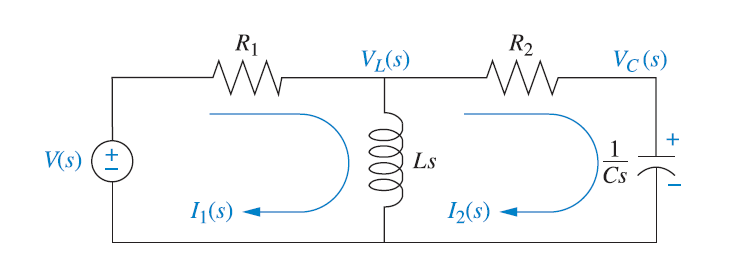
\includegraphics{mesh3.png} The transfer function relating $I_2(s)$ to $V$ is $\frac{LCs^2}{LCs^2(R_1 + R_2) + s(R_1R_2C + L) + R_1}$}
\subsubsection{Mesh Analysis}
\begin{proof}
	By the first loop
	\[V(s) = R_1I_1(s) + Ls(I_1(s) - I_2(s))\] and by the second 
	\[0 = R_2I_2(s) + \frac{1}{Cs}I_2(s) + Ls(I_2(s) - I_1(s))\]
	using Kirchhoff's voltage law. In the language of matrices
	\[\begin{bmatrix}
		R_1 + Ls & -Ls \\
		-Ls & R_2 + \frac{1}{Cs} + Ls 
	\end{bmatrix} \begin{bmatrix}
	I_1(s) \\ I_2(s)
\end{bmatrix} = \begin{bmatrix}
V(s) \\ 0
\end{bmatrix}\] so by Cramer's Rule
\[I_2(s) = \frac{\abs{\begin{bmatrix}
			R_1 + Ls & V(s) \\ -Ls & 0
\end{bmatrix}}}{\abs{\begin{bmatrix}
R_1 + Ls & -Ls \\ -Ls & R_2 + \frac{1}{Cs} + Ls 
\end{bmatrix}}}\]
\[= \frac{LsV(s)}{(R_1 + Ls)(R_2 + \frac{1}{Cs} + Ls) - L^2s^2} =  \frac{LsV(s)}{R_1R_2 + \frac{R_1}{Cs} + R_1Ls + LsR_2 + \frac{Ls}{Cs} + L^2s^2 - L^2s^2}\]
\[ =  \frac{CLs^2V(s)}{CsR_1R_2 + R_1 + CsR_1Ls + CsLsR_2 + Ls}\]
and so 
\[\frac{I_2(s)}{V(s)} =  \frac{CLs^2}{CsR_1R_2 + R_1 + CsR_1Ls + CsLsR_2 + Ls}\]
\end{proof}
 \subsubsection{(Nodal Analysis) Find $\frac{V_C(s)}{V(s)}$}
 \begin{proof}
 	By the currents at node $V_L(s)$
 	\[ -\frac{V_L(s)}{Ls} + \frac{V(s) - V_L(s)}{R_1} - \frac{V_L(s) - V_C(s)}{R_2}= 0 \iff V_C(s)\frac{1}{R_2} + V(s)\frac{1}{R_1} = \frac{V_L(s)}{Ls} + \frac{V_L(s)}{R_1} + \frac{V_L(s)}{R_2}\]
 	and by those at node $V_C(s)$
 	\[\frac{V_C(s)}{1/Cs} - \frac{V_L(s) - V_C(s)}{R_2} = 0 \iff V_C(s)(Cs + \frac{1}{R_2}) =  \frac{V_L(s)}{R_2}\]
 	In the language of matrices
 	\[\begin{bmatrix}
 		\frac{1}{R_2} & \frac{1}{R_1} \\
 		Cs + \frac{1}{R_2} & 0 
 	\end{bmatrix} \begin{bmatrix}
 	V_C(s) \\ V(s)
 \end{bmatrix} = V_L(s)\begin{bmatrix}
 \frac{1}{Ls} + \frac{1}{R_1} + \frac{1}{R_2} \\ \frac{1}{R_2}
\end{bmatrix}\]
Using Cramer's Rule
\[V_C(s) = V_L(s)\frac{\abs{\begin{bmatrix}
	\frac{1}{Ls} + \frac{1}{R_1} + \frac{1}{R_2} & \frac{1}{R_1} \\ \frac{1}{R_2} & 0		
\end{bmatrix}}}{\abs{\begin{bmatrix}
\frac{1}{R_2} & \frac{1}{R_1} \\
Cs + \frac{1}{R_2} & 0 
\end{bmatrix}}}\]
\[= V_L(s)\frac{\frac{1}{R_2}}{Cs + \frac{1}{R_2}} = V_L(s)\frac{1}{CsR_2 + 1}\]
and
\[V(s) = V_L(s)\frac{\abs{\begin{bmatrix}
				\frac{1}{R_2} & \frac{1}{Ls} + \frac{1}{R_1} + \frac{1}{R_2} \\
			Cs + \frac{1}{R_2} & \frac{1}{R_2}
\end{bmatrix}}}{\abs{\begin{bmatrix}
			\frac{1}{R_2} & \frac{1}{R_1} \\
			Cs + \frac{1}{R_2} & 0 
\end{bmatrix}}}\]
\[= V_L(s) \frac{\frac{1}{R_2^2} - \frac{C}{L} - \frac{1}{LsR_2} - \frac{Cs}{R_1} - \frac{1}{R_1R_2} - \frac{Cs}{R_2} - \frac{1}{R_2^2}}{-\frac{Cs}{R_1} - \frac{1}{R_1R_2}}\]

\[= V_L(s) \frac{ \frac{C}{L} + \frac{1}{LsR_2} + \frac{Cs}{R_1} + \frac{1}{R_1R_2} + \frac{Cs}{R_2}}{\frac{Cs}{R_1} + \frac{1}{R_1R_2}}\]

\[= V_L(s) \frac{ R_1R_2Cs + R_1 + R_2CLs^2 + Ls + R_1CLs^2 }{R_2CLs^2 + Ls}\]
thus 
\[\frac{V_C(s)}{V(s)} = \frac{R_2CLs^2 + Ls}{(CsR_2 + 1)( R_1R_2Cs + R_1 + R_2CLs^2 + Ls + R_1CLs^2)}\]
\[= \frac{Ls}{ R_1R_2Cs + R_1 + R_2CLs^2 + Ls + R_1CLs^2 }\]
\[= \frac{Ls}{ s^2(R_1CL + R_2CL) + s(R_1R_2C + L)  + R_1 }\]
 \end{proof}

\subsubsection{Norton Equivalent (Nodal Analysis with Admittances): \newline 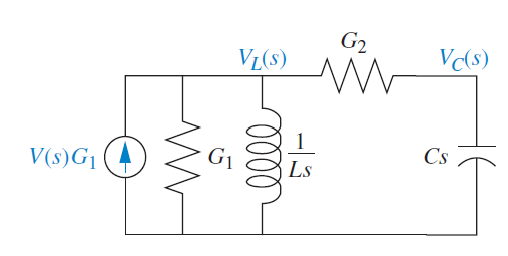
\includegraphics{mesh4.png}}
\begin{proof}
	At $V_L(s)$
	\[V(s)G_1 = G_1V_L(s) + \frac{1}{Ls}V_L(s) + G_2(V_L(s) - V_C(s))\]
	and at $V_C(s)$
	\[0 = -G_2(V_L(s) + V_C(s)) + CsV_C(s)\]
\end{proof}



\end{document}
